\section*{Robotic arm}
\subsection*{Forward kinematics}
\subsection*{Inverse kinematics}


%%%%%%%%%%%%%%%%%%

\section*{Base}

 The motors will be connected to tracks on the robot and can therefore be modelled as two wheels connected with a rod, as seen in figure \ref{fig:base_math_model}.\\ 
This means that most of the mathematical modeling is very straight forward given that we can read the encoders from the motors. From the encoders we would be able to get both the length the robot has traveled and more importantly the individual speed each motor rotates with. The speed for the individual motor is of course given by: 

\begin{equation}
    v_m=\frac{2\pi r_{wheel}/N_{encoders}}{\Delta t}
    \label{eq:base_system_eq1}
\end{equation}

\noindent Where $N_{encoders}$ is the number of encoders on the motor, $r_{wheel}$ is the radius of the driving wheel and thickness of the track and $\Delta t$ is the time between the previous encoder reading and the most recent one. By doing this for both the left and right motor we can find how fast the robot is moving along the line by:

\begin{equation}
    \overline{v}= \frac{v_L+v_R}{2}(-\cos \theta \hat{i}+ \sin \theta \Hat{j})
\end{equation}

\noindent Where the $y$-axis parallel to the line. In a similar fashion to how we calculated the velocity of the robot, the rate of change of the angle can be calculated using:

\begin{equation}
    \Dot{\theta} = \frac{v_R-v_L}{2r_{base}}
    \label{eq:base_system_eq2}
\end{equation}

\noindent Where $r_{base}$ is the distance from the center of the base to the wheels. From this and figure \ref{fig:base_math_model} it's easy to see that the change of angle then becomes:

\begin{equation}
    \theta = sin^{-1}\left(\frac{V_L-V_R}{2r_{base}}t\right)
\end{equation}

\begin{figure}[H]
    \centering
    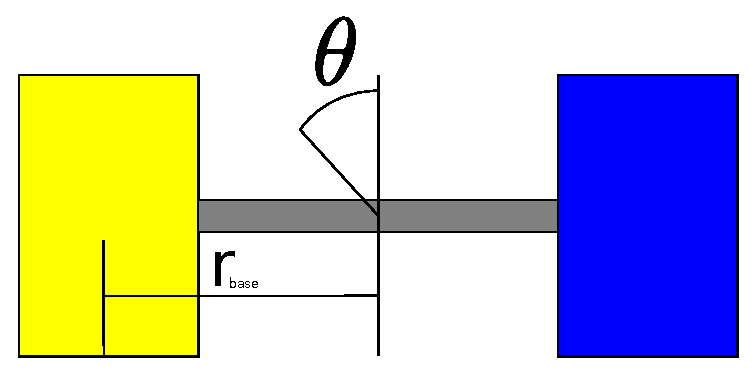
\includegraphics[width=0.7\textwidth]{base_math_model.eps}
    \caption{Modelling of the base as two wheels connected with a rod, where $\theta$ is the angle to the line}
    \label{fig:base_math_model}
\end{figure}

Given small angles \footnote{Which will be assumed because the robot will be operating on a grid with hard coded functions for turning at QR-codes}, we can therefore write this as:

\begin{equation}
    \theta = \frac{V_L-V_R}{2r_{base}}t
\end{equation}


\noindent Using equations \eqref{eq:base_system_eq1}-\eqref{eq:base_system_eq2} a system can be built for simulations in matlab, using rate of change and max/min value limiters for simulations of the motors physical restrictions.

%%%%%%%%%%%%%%%%%%%%%%%%%%%%%%%%%


\section*{Camera vision and calibration}
In this section it is outlined the theory behind the camera vision system. 
How points in a 3D-space are projected on a 2D-plane, calibration and distortion correction. 
\subsection*{Camera model}
\subsection*{Distortion}
